\documentclass[12pt]{article}

\usepackage{pablo-devoir}
\usepackage{pablo-listings}
\usepackage[a5paper,margin=2cm]{geometry}

\pagestyle{empty}

\title{{\small (In)Équation --- Espace}\\ Corrigé}
\date{5/11/14}
\classe{2\up{des}14}
\dsnum{DS 2}

\begin{document}

\maketitle

\begin{exercice}[Développement et Factorisation --- 6 points]
  \emph{On considère la fonction définie par $f(x)=\left( x+1 \right)^2+\left( x+1 \right)\left( x-2 \right)$.}

  \begin{enumerate}[(1)]
    \item \begin{enumerate}

        \item \emph{Montrer que $f(x)=\left( x+1 \right)\left( 2x-1 \right)$.}
          Il y a différentes manières de faire (l'une d'entre elle est de développer toutes les expressions pour montrer qu'on obtient même chose). En voici une obtenue en factorisant par $x+1$.
          \begin{align*}
            f(x)&=\left( x+1 \right)^2+\left( x+1 \right)\left( x-2 \right)\\
            &=\left( x+1 \right)\left[\left( x+1 \right)+\left( x-2 \right)\right]\\
            &=\left( x+1 \right)\left[ x+1+x-2 \right]\\
            &=\left( x+1 \right)\left( 2x-1 \right)
          \end{align*}
        \item \emph{Montrer que $f(x)=2x^2+x-1$.} On part de l'expression $f(x)=\left( x+1 \right)\left( 2x-1 \right)$ (nous aurions tout aussi bien partir de l'expression originale, mais les calculs sont un peu plus simples comme cela).
          \begin{align*}
            f(x) &= \left( x+1 \right)\left( 2x-1 \right)\\
            &= x\times2x+x\times\left( -1 \right)+1\times2x+1\times\left( -1 \right)\\
            &= 2x^2+x-1
          \end{align*}
      \end{enumerate}
    \item \begin{enumerate}
          \pagebreak
        \item \emph{Résoudre $f(x)=0$.} On part de l'expression $f(x)=\left( x+1 \right)\left( 2x-1 \right)$ :
          \begin{align*}
            f(x) &=0\\
            \left( x+1 \right)\left( 2x-1 \right) &=0\\
            x+1=0 &\text{ ou } 2x-1=0\\
            x=-1 &\text{ ou } 2x=1\\
            x=-1 &\text{ ou } x=\frac{1}{2}
          \end{align*}
        \item \emph{Résoudre $f(x)=-1$.}
          \setlength{\columnseprule}{1pt}
          \begin{multicols}{2}
            Nous partons cette fois de l'expressions développée de $f$.
          \begin{align*}
            2x^2+x-1 &= -1\\
            2x^2+x &= -1+1\\
            2x^2+x &= 0\\
            x\left( 2x+1 \right) &=0\\
          \end{align*}
          C'est une équation produit, qui donne :
          \begin{align*}
            x=0 &\text{ ou } 2x+1=0\\
            x=0 &\text{ ou } 2x=-1\\
            x=0 &\text{ ou } x=-\frac{1}{2}
          \end{align*}
    \end{multicols}
      \end{enumerate}
  \end{enumerate}
\end{exercice}

\begin{exercice}[Inéquations --- 6 points]
  \emph{Résoudre (si nécessaire) chacun des couples d'inéquations suivant, et présenter les solutions sur la droite des réels, puis sous forme d'intervalle.}
  \begin{enumerate}[(1)]
    \item
          \setlength{\columnseprule}{0pt}
      \begin{multicols}{2}
        \begin{align*}
          2x+1 &> 3+x \\
          2x -x &> 3-1\\
          x&>2
        \end{align*}
        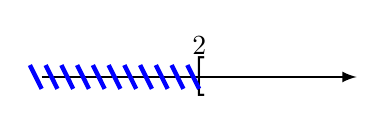
\begin{tikzpicture}[thick]
          \draw[-latex] (0,0) -- (4,0);
          \draw ( 2,0) node{{\Large\textbf{[}}} node[above=1ex]{$2$};
          \foreach \i in {0, .2, ..., 2} {
            \draw[blue, ultra thick] (\i,-1ex) -- ({\i-.15},1ex);
          }
        \end{tikzpicture}
      \end{multicols}
      \pagebreak
    \item 
      \begin{multicols}{2}
        $x<2$ ou $x>3$

        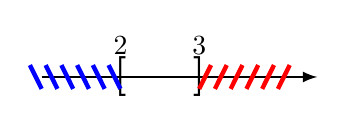
\begin{tikzpicture}[thick]
          \draw[-latex] (1,0) -- (4.5,0);
          \draw ( 2,0) node{{\Large\textbf{[}}} node[above=1ex]{$2$};
        \draw ( 3,0) node{{\Large\textbf{]}}} node[above=1ex]{$3$};
        \foreach \i in {1, 1.2, ..., 2} {
          \draw[blue, ultra thick] (\i,-1ex) -- ({\i-.15},1ex);
        }
        \foreach \i in {3, 3.2, ..., 4} {
          \draw[red, ultra thick] (\i,-1ex) -- ({\i+.15},1ex);
        }
      \end{tikzpicture}
    \end{multicols}

  Puisque l'opérateur est « ou », les solutions sont les parties de la droite qui sont hachurées \emph{au moins une fois}. Les solutions sont donc : $x\in\left]-\infty;2\right[\cup\left]3;+\infty\right[$.
  \item 
    \begin{multicols}{2}
      $x<3$ et $x>2$

      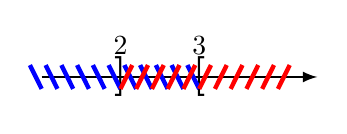
\begin{tikzpicture}[thick]
        \draw[-latex] (1,0) -- (4.5,0);
      \draw ( 2,0) node{{\Large\textbf{]}}} node[above=1ex]{$2$};
      \draw ( 3,0) node{{\Large\textbf{[}}} node[above=1ex]{$3$};
      \foreach \i in {1, 1.2, ..., 3} {
        \draw[blue, ultra thick] (\i,-1ex) -- ({\i-.15},1ex);
      }
      \foreach \i in {2, 2.2, ..., 4} {
        \draw[red, ultra thick] (\i,-1ex) -- ({\i+.15},1ex);
      }
    \end{tikzpicture}
  \end{multicols}

Puisque l'opérateur est « et », les solutions sont les parties de la droite qui sont hachurées \emph{deux fois}. Les solutions sont donc : $x\in\left]2;3\right[$.
  \end{enumerate}
\end{exercice}

\begin{exercice}[Volume --- 6 points]~
  \begin{multicols}{2}
    \begin{em}
      Un fleuriste souhaite connaître le volume d'un vase qu'il utilise. Ce vase a la forme d'un cône tronqué, c'est-à-dire d'un cône auquel on a enlevé la partie inférieure (voir ci-contre).

      Le rayon du cercle supérieur est 10~cm, celui du cercle inférieur est 6~cm, et les hauteurs sont indiquées sur le schéma.
    \end{em}

    \columnbreak

    \begin{center}
      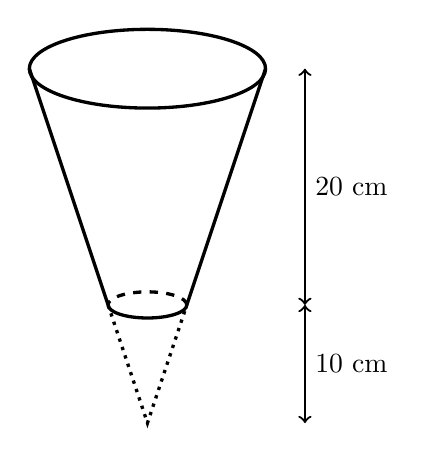
\begin{tikzpicture}[very thick]
        \draw[] (1,0) -- (0,3);
        \draw[] (2,0) -- (3,3);
        \draw[] (1.5,3) ellipse (1.5 and 0.5);
        \draw[dashed] (2,0) arc (0:180:0.5 and 0.166);
        \draw[] (1,0) arc (180:360:0.5 and 0.166);

        \draw[dotted] (1,0) -- (1.5,-1.5) -- (2,0);

        \draw[thick,<->] (3.5,3)
        -- (3.5,0)    node[midway,right]{20~cm};
        \draw[thick,<->] (3.5,0)
        -- (3.5,-1.5) node[midway,right]{10~cm};
      \end{tikzpicture}
    \end{center}
  \end{multicols}

  \emph{Les résultats seront arrondis au dixième.}

  \begin{enumerate}[(1)]
    \item \emph{Calculer le volume du grand cône (avant suppression de la partie tronquée).}
      
      La formule du volume d'un cône de révolution est $\frac{1}{3}\pi r^2h$ (où $r$ est le rayon de la base, et $h$ la hauteur). Donc le volume du grand cône est : $\frac{1}{3}\pi\times10^2\times30=1000\pi=3141,6cm^3$.
    \item \emph{Calculer le volume de la partie tronquée (en pointillés sur la figure).}
      
      Ce volume est $\frac{1}{3}\pi\times6^2\times10=120\pi=377,0cm^3$.
    \item \emph{En déduire le volume du vase.}
      
      Le volume du vase est la différence des deux volumes, soit $3141,6-377,0=2764,6cm^3$.
  \end{enumerate}

\end{exercice}

\begin{exercice}[Problème ouvert --- 2 points]
  \begin{multicols}{2}
    \noindent \emph{On considère le cube $ABCDEFGH$, de côté 2~cm. Le point $I$ est le centre de la face $AEFB$ ; $J$ est le centre de la face $CGFB$. Quelle est la longueur du segment $[IJ]$ ?}

    \begin{center}
      \begin{tikzpicture}[scale=2,line width=1pt]
        \coordinate (O) at (0,0);
        \coordinate (x) at (1,0);
        \coordinate (y) at ({0.8*cos(30)},{0.8*sin(30)});
        \coordinate (z) at (0,1);

        \coordinate (A) at (O);
        \coordinate (B) at ($(O) + (x)$);
        \coordinate (C) at ($(O) + (x) + (y)$);
        \coordinate (D) at ($(O) + (y)$);
        \coordinate (E) at ($(O) + (z)$);
        \coordinate (F) at ($(O) + (z) + (x)$);
        \coordinate (G) at ($(O) + (z) + (x) + (y)$);
        \coordinate (H) at ($(O) + (z) + (y)$);
        \coordinate (I) at ($(O) + 0.5*(x) + 0.5*(z)$);
        \coordinate (J) at ($(O) + (x) + 0.5*(y) + 0.5*(z)$);

        \draw (A) node[below left]{$A$};
        \draw (B) node[below right]{$B$};
        \draw (C) node[right]{$C$};
        \draw (D) node[below]{$D$};
        \draw (E) node[left]{$E$};
        \draw (F) node[above]{$F$};
        \draw (G) node[right]{$G$};
        \draw (H) node[above]{$H$};
        \draw (A) -- (B) -- (C) -- (G) -- (H) -- (E) -- (F) -- (B);
        \draw (A) -- (E);
        \draw (F) -- (G);
        \draw[dashed] (D) -- (H);
        \draw[dashed] (D) -- (A);
        \draw[dashed] (D) -- (C);

    %\draw[dotted] (A) -- (F) -- (C);
        \draw (I) node{$\times$} node[above left]{$I$};
        \draw (J) node{$\times$} node[above right]{$J$};
        \draw[dotted] (I) -- (J);

        % Solution
        \draw (A) -- (F) -- (C);
        \draw[dashed] (A) -- (C);
      \end{tikzpicture}
    \end{center}
  \end{multicols}

  \emph{Il y a différentes manières de résoudre ce problème. En voici une.}

  On se place dans le triangle $AFC$ : $I$ est le milieu de $[AF]$, et $J$ le milieu de $[FC]$, donc d'après l'énoncé des mileux, $IJ=\frac{AC}{2}$. Reste à calculer $AC$.

  On se place dans le triangle $ABC$. Puisque $ABCDEFGH$ est un cube de côté 2~cm, $ABCD$ est un carré de côté 2~cm, et $ABC$ est un triangle rectangle en $B$. Nous appliquons donc le théorème de Pythagore : $AB^2+BC^2=AC^2$, donc $2^2+2^2=AC^2$, et $8=AC^2$. Donc $AC=\sqrt{8}=2\sqrt{2}$.

  Donc $IJ=\frac{AC}{2}=\frac{2\sqrt{2}}{2}=\sqrt{2}$ : la longueur $IJ$ est égale à $\sqrt{2}$~cm, soit environ $1,41$~cm.

\end{exercice}
\end{document}
